\section{Chapter introduction}

This chapter presents the preliminary work to evaluate and calibrate the new \native routing scheme before running coupled simulations with ICOLMDZOR. As a reminder, the pre-existing version of the routing scheme, \std, cannot be used with ICOLMDZOR because it imposes constraints on the ORCHIDEE and routing grids that are incompatible with the icosahedral grid. 
The \native routing is based on the same physical principles (described in Chapter \ref{chap:methods}) as \std but it involves an additional piece of code to interpolate between the ORCHIDEE grid and the routing grid, and other changes to make it compatible with any DEM and ORCHIDEE grid.

Two objectives were initially identified:
\begin{itemize}
    \item Ensure that the \native code could replicate the general behaviour and quantitatively match the simulated reservoir volumes and river discharge of \std, if given the same parameters and DEM as input. 
    \item Evaluate and calibrate \native using a high resolution DEM over the Iberian Peninsula to identify an appropriate set of parameters for coupled simulations.
\end{itemize}

However, this work raised more general scientific questions, which were addressed using offline simulations with different experimental setups. Apart from the hypothesis that horizontal transfers of groundwater between routing grid cells are not represented and the technical need to respect the Courant-Friedrichs-Lewy condition, the routing modelling principles are theoretically independent of the spatial and temporal resolution. In practice however, switching from a 0.5° to a 1-arcminute resolution DEM seems to affect the results and require changes in the choice of parameters \citep{kilic_evaluation_2023}. During the parameter tuning, which used discharge observations as a reference, the relative importance of various factors was also analysed, such as the meteorological forcing used and the activation of irrigation. It also raised the question of how the irrigation scheme could be adapted to better match regional practices and achieve more realistic values of river discharge in irrigated river basins. Finally, an important question was the impact and strength of the interdependency between irrigation, the water volume in the river reservoir and simulated river discharge in large basins.

\section{Methods and data}

The relevant routing outputs for evaluation and parameter tuning are river discharge and water volumes in each of the reservoirs (groundwater, overland, rivers). 
These volumes, however, cannot be easily compared to observations, since large-scale measurements of groundwater or river volumes are complex and may not physically correspond to the conceptual level of the reservoirs modelled in ORCHIDEE.
Their importance in this work is mainly justified by the fact that the irrigation scheme withdraws water from these reservoirs to satisfy the irrigation demand while conserving water.

All simulations for this chapter were run in offline mode with the setup and input data described in Chapter \ref{chap:methods}.
Most simulations were run from 2000 to 2012, with the WATCH Forcing Data ERA-Interim \citep[WFDEI, ][]{weedon_wfdei_2014}. Sensitivity experiments to assess the impact of the forcing were also run with the Global Soil Wetness Project Phase 3 Atmospheric Boundary Conditions \citep[GSWP3, ][]{kim_hyungjun_global_2017}, another forcing dataset which is only available until 2010.
In all simulations, to allow the vegetation and hydrological variables to reach an equilibrium with the local climate, the first three years were considered as a warm-up and removed from the analysis, thus restricted to 10 years (2003-2012) for the WFDEI forcing. The regional domain covers the Iberian Peninsula and part of Morocco, since at the time, this region was also considered as a study area for coupled simulations. Since this idea was not pursued, the analysis only focuses on the Iberian Peninsula.
Topographical data from the two DEMs presented in Chapter \ref{chap:methods} was used, either from the 0.5°-resolution DEM historically associated with the \std routing or from the MERIT DEM at 2-km resolution.

In all this chapter, the simulated river discharge is evaluated against monthly observation data from discharge stations of the Global Runoff Data Center \citep[GRDC, https://grdc.bafg.de,][]{fekete_global_2003}.
Stations were positioned on the 0.5° DEM grid using only the GPS position, and on the MERIT DEM grid with tools presented in \cite{polcher_hydrological_2023}, which use the GPS position of the stations as well as the upstream catchment area to find the most appropriate grid cell for comparison with the observations. 
Four stations were selected, which are all on large rivers (Ebro, Douro, Tagus, Guadiana) and present a 100\% coverage over the period 2003-2012. They all show large discharge values, meaning they represent the integrated discharge over a large share of the basins. They are shown on Fig. \ref{fig:halfdeg_stations_map} and their characteritics (including error on the positionning) are given in Table \ref{tab:error_metrics}.

\begin{figure}[htbp]
    \centering
    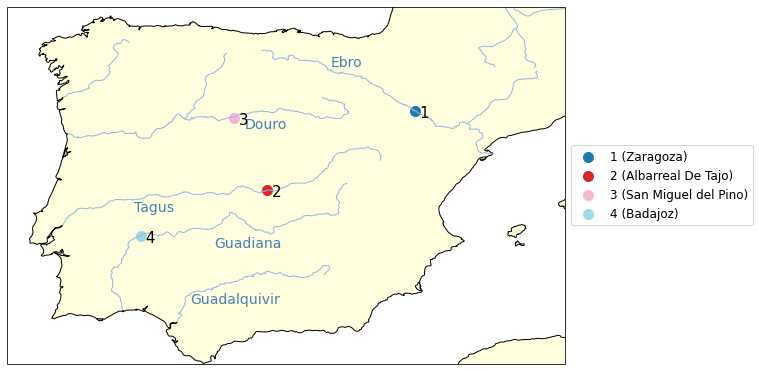
\includegraphics[width=0.7\textwidth]{images/chap3/river_discharge/halfdeg_4stations_map.png}
    \caption{Discharge stations selected for the routing scheme evaluation and parameter tuning.}
    \label{fig:halfdeg_stations_map}
\end{figure}

\begin{table}[hbtp]
    \centering
    \caption{Characteristics of river discharge stations used for the routing scheme evaluation and parameter tuning.}
    \resizebox{\textwidth}{!}{%
        \begin{tabular}{lccccc}
        \hline
        \textbf{Station} & \textbf{Altitude (m)} & \textbf{River} & \textbf{Area (km$^2$)} & \textbf{Distance error (km)} & \textbf{Area error} \\
        \hline
        1 (Zaragoza)             & 189 & Ebro     & 40434 & 0.505 & 0.0047 \\
        2 (Albarreal de Tajo)    & 430 & Douro    & 27159 & 0.978 & 0.0127 \\
        3 (San Miguel del Pino)  & 670 & Tagus    & 36570 & 0.660 & 0.0014 \\
        4 (Badajoz)              & 166 & Guadiana & 48530 & 0.895 & 0.0046 \\
        \hline
    \end{tabular}
    }
    \label{tab:error_metrics}
\end{table}
%option:add mean discharge when doing metrics

\section{Consistency of \native with \std routing}
\label{sec:routing_consistency}
\subsection{Simulation experiments}

This first analysis used the \native routing in the same setup as the \std routing. The meteorological forcing is WFDEI, and the input DEM was the same (0.5° resolution), and the time constants for the three reservoirs were the same as the default values for the global model (Table \ref{table:tcst_consistency}).
Four simulations were run, two without irrigation (labeled as \textit{no\_irr}) to assess the routing schemes without its influence, and two with irrigation (labeled as \textit{irr}). It must be noted that these simulations were not aimed at evaluating the realism of simulated irrigation or discharge (which will be addressed in Section \ref{section:calib}) but only to assess if the new routing code behaves similarly in the two versions.

\begin{table}[h]
\centering
\begin{tabular}{|c|c|c|}
\hline
\textbf{TCST\_SLOW} & \textbf{TCST\_FAST} & \textbf{TCST\_STREAM} \\ \hline
25            & 3             & 0.24            \\ \hline
\end{tabular}
\caption{Routing time constant for the consistency analysis ($day \cdot km^{-1}$).}
\label{table:tcst_consistency}
\end{table}

\subsection{Case of coastal grid cells}
\label{sec:coastal_grid_cells}

%figure : 12 maps of mean reservoir volumes and hydrographs, for both sims and diff
\begin{figure}[htbp]
    \centering
    \makebox[\linewidth]{
        \begin{minipage}{1.25\linewidth}
            \begin{tabular}{ccc}
                \begin{subfigure}[b]{0.33\linewidth}
                    \caption{Groundwater reservoir\\(annual mean, \std)}
                    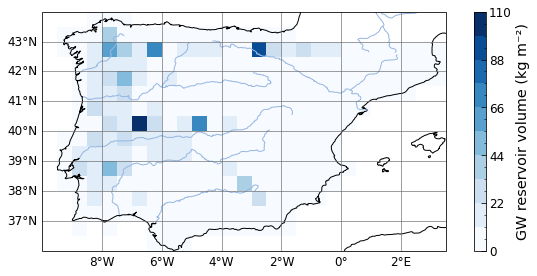
\includegraphics[width=\textwidth]{images/chap3/maps/slowr_subgrid.png}
                \end{subfigure} &
                \begin{subfigure}[b]{0.33\linewidth}
                    \caption{Groundwater reservoir\\(annual mean, \native)}
                    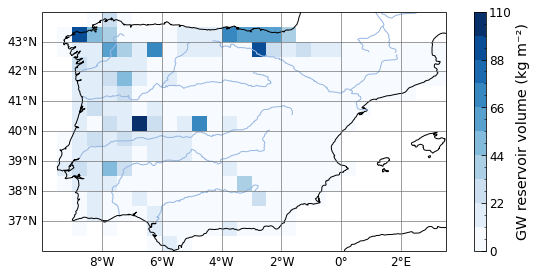
\includegraphics[width=\textwidth]{images/chap3/maps/slowr_interp.png}
                \end{subfigure} &
                \begin{subfigure}[b]{0.33\linewidth}
                    \caption{Groundwater reservoir difference\\ (\native -\std)}
                    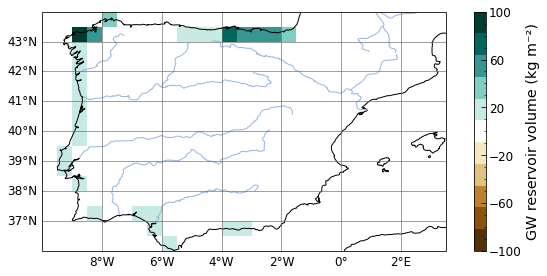
\includegraphics[width=\textwidth]{images/chap3/maps/slowr_diff.png}
                \end{subfigure} \\
                
                \begin{subfigure}[b]{0.33\linewidth}
                    \caption{Overland reservoir\\(annual mean, \std)}
                    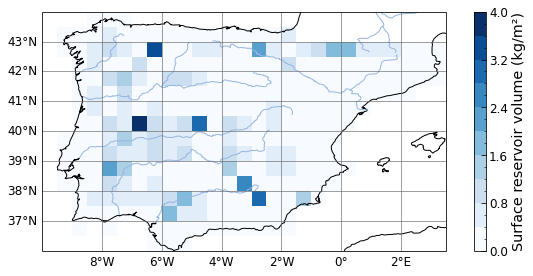
\includegraphics[width=\textwidth]{images/chap3/maps/fastr_subgrid.png}
                \end{subfigure} &
                \begin{subfigure}[b]{0.33\linewidth}
                    \caption{Overland reservoir\\(annual mean, \native)}
                    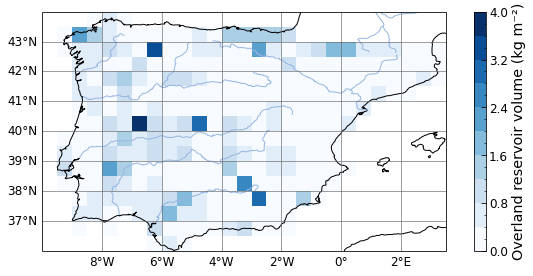
\includegraphics[width=\textwidth]{images/chap3/maps/fastr_interp.png}
                \end{subfigure} &
                \begin{subfigure}[b]{0.33\linewidth}
                    \caption{Overland reservoir difference\\ (\native -\std)}
                    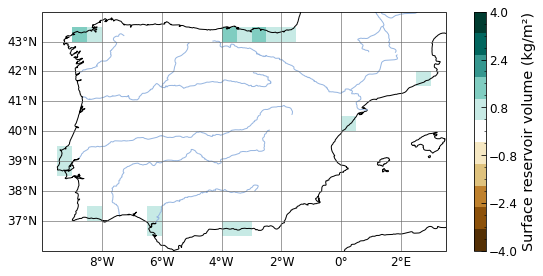
\includegraphics[width=\textwidth]{images/chap3/maps/fastr_diff.png}
                \end{subfigure} \\
                
                \begin{subfigure}[b]{0.33\linewidth}
                    \caption{River reservoir\\(annual mean, \std)}
                    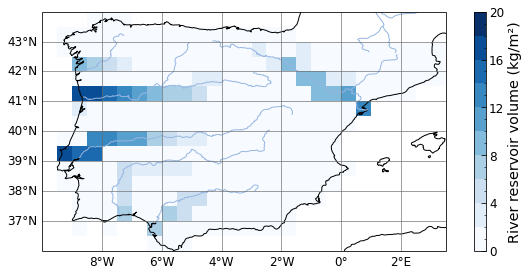
\includegraphics[width=\textwidth]{images/chap3/maps/streamr_subgrid.png}
                \end{subfigure} &
                \begin{subfigure}[b]{0.33\linewidth}
                    \caption{River reservoir\\(annual mean, \native)}
                    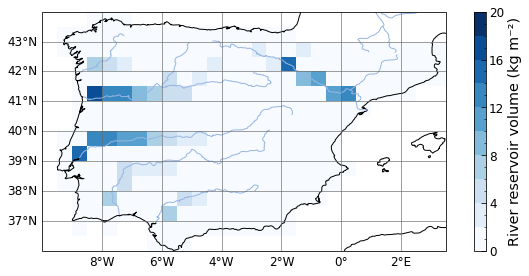
\includegraphics[width=\textwidth]{images/chap3/maps/streamr_interp.png}
                \end{subfigure} &
                \begin{subfigure}[b]{0.33\linewidth}
                    \caption{River reservoir difference \\(\native -\std)}
                    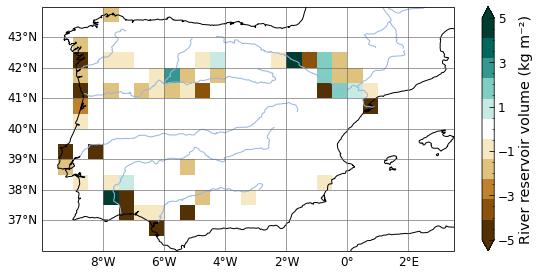
\includegraphics[width=\textwidth]{images/chap3/maps/streamr_diff.png}
                \end{subfigure} \\
                
                \begin{subfigure}[b]{0.33\linewidth}
                    \caption{River discharge\\(annual mean, \std)}
                    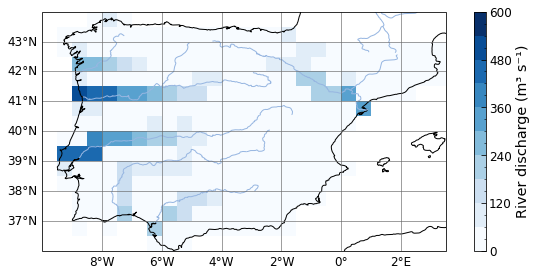
\includegraphics[width=\textwidth]{images/chap3/maps/hydrographs_subgrid.png}
                \end{subfigure} &
                \begin{subfigure}[b]{0.33\linewidth}
                    \caption{River discharge\\(annual mean, \native)}
                    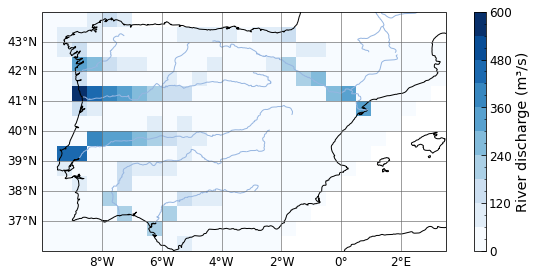
\includegraphics[width=\textwidth]{images/chap3/maps/hydrographs_interp.png}
                \end{subfigure} &
                \begin{subfigure}[b]{0.33\linewidth}
                    \caption{River discharge difference \\(\native -\std)}
                    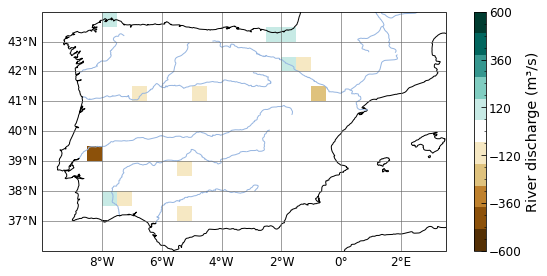
\includegraphics[width=\textwidth]{images/chap3/maps/hydrographs_diff.png}
                \end{subfigure} \\
            \end{tabular}
        \end{minipage}
    }
    \caption{Annual mean (2003-2012) of reservoir volumes and river discharge for \std (\noirr), \native (\noirr) and difference between them.}
    \label{fig:routing_reservoirs_halfdeg}
\end{figure}

The comparison of the mean volumes for the groundwater and overland reservoirs (Fig. \ref{fig:routing_reservoirs_halfdeg}a-f) shows differences only on coastal grid cells (which was verified not to be an artefact of the colour map used), with very low volumes in \std that can become large in \native, particularly in the northern strip of the Peninsula. Considering these are mostly mountainous regions which receive large precipitation, and therefore exhibit high drainage and surface runoff, the values computed by \native in this region are in the expected order of magnitude compared to neighbouring non-coastal grid cells, whereas the values in \std are 10 to 70 times smaller.
Therefore, the most likely explanations to the differences are that either \std does not receive all the water from runoff and drainage, or it does not hold water in the reservoirs of these coastal grid cells as long as it should. 
In the routing scheme, coastal grid cells have to be managed differently since they must flow to the sea rather than to the river reservoir of the downstream grid cell. It is therefore possible that different modelling or implementation choices were made when developing the code for \std and \native.
In particular, a different treatment of the land-sea mask could lead to either a different regridding of runoff and drainage that sends part of the water directly to the sea, or to different $topoindex$ values in coastal grid cells that empty the reservoir faster than expected.
However these discrepancies are still not completely understood and still under investigation, in collaboration with Antoine Bierjon (research engineer at IPSL), to clarify their cause and determine whether they introduced errors or corrected existing flaws of the previous code for coastal grid cells.

%old possible explanation with Contfrac, further tested and doesn't seem to be the problem...
% These differences are thought to be the consequence of a different handling of water quantities and their units in \native compared to \std. 
% As detailed in Section \ref{sec:irrig_interp_variables}, in \native, drainage and surface runoff are computed on the ORCHIDEE grid, in $kg \cdot m^{-2}$ (equivalent to $mm$ over the grid cell) and converted to absolute water quantities (in $kg$) before being interpolated to the DEM grid. These absolute quantities are routed on the DEM grid and the new water quantities in the reservoirs are reinterpolated to the ORCHIDEE grid (even when the two grids have the same resolution). To express them as an areal value, in $kg \cdot m^{-2}$, the absolute water quantity has to be divided by the area of the grid cell. It is considered likely that this back-and-forth interpolation and change of units introduces the differences, by accounting for continental fraction (to obtain the exact area on coastal points) whereas in \std this was not necessary since all computations were on the same grid cell. Such subtleties in the code were introduced to enable compatibility with any DEM grid.

Since this issue affected only the groundwater and overland reservoirs and was located only on coastal grid cells, it was considered that for the purpose of this work, the impacts should not affect the results substantially and that \native could be used in its current version.

\hfill

Regarding the river reservoir (Fig. \ref{fig:routing_reservoirs_halfdeg}g-i), a new modelling choice was made on coastal grid cells. In \std, there was a river reservoir for these grid cells, whereas it was removed in \native as schematized in Fig. \ref{fig:coastal_routing_behaviour}. This choice was made during the development of the code and might be changed in future versions to ensure consistency with the other two reservoirs. It is responsible for the lower volumes of the river reservoirs of the large river outlets in \native (Fig. \ref{fig:routing_reservoirs_halfdeg}i).

However, this difference does not translate to values of river discharge since it is still computed in coastal grid cells in \native using the outflow from the river reservoir of the upstream grid cells, and from the groundwater and overland reservoirs (Fig. \ref{fig:routing_reservoirs_halfdeg}j-l). River discharge is larger in \native than in \std on all coastal grid cells (Fig. \ref{fig:routing_reservoirs_halfdeg}l). This is very likely the consequence of the differences noticed in the groundwater and overland reservoir, which both contribute to the discharge and are much larger in \native for coastal grid cells, as explained previously.

% The way to compute river discharge in these coastal points is also slightly different in \native, as it includes the flow from the river reservoir of the upstream grid cell, as well as the flow from the groundwater and overland reservoirs of the grid cell, whereas drainage and surface runoff were considered to flow directly in the ocean in \std. This explains why discharge values are or similar order of magnitude but larger in \native (Fig. \ref{fig:routing_reservoirs_halfdeg}l). Figure \ref{fig:coastal_routing_behaviour} schematizes the differences in implementation that explain the differences seen in the river reservoir and in the discharge on coastal grid cells.

\begin{figure}[htbp]
    \centering
    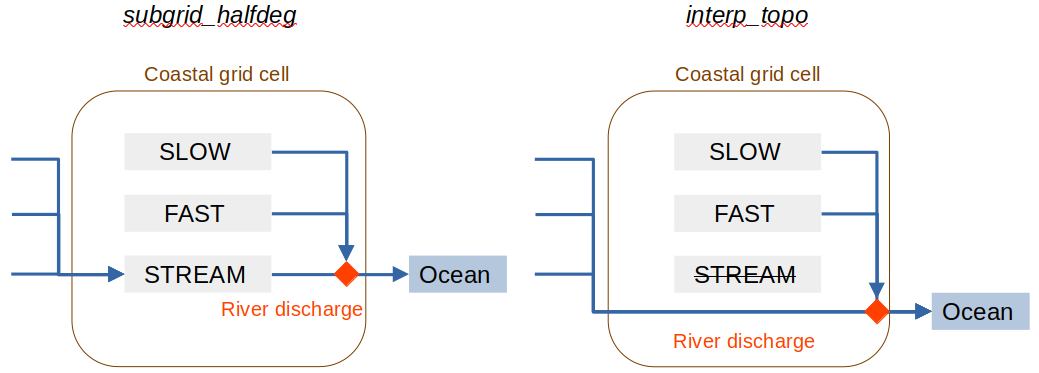
\includegraphics[width=\textwidth]{images/chap3/coastal_routing_behaviour_v3.png
}
    \caption{Differences in implementation between \std and \native on coastal grid cells.}
    \label{fig:coastal_routing_behaviour}
\end{figure}

\subsection{Routing path and average impacts on reservoir volumes}
Apart from coastal grid cells, the most noticeable discrepancy between the two routing versions concerns the river reservoir and river discharge, with differences which can be either positive or negative in some non-coastal points. It can be seen in Fig. \ref{fig:routing_reservoirs_halfdeg}j-l particularly that the water does not exactly follow the same path, meaning that the DEM is not interpreted exactly in the same way. 
This is attributed to the DEM preprocessing implemented in \std, mentioned in Section \ref{section:routing_methods}, which are specific to its structure and therefore not implemented in \native. In the large rivers where there are differences, \native seems to use shorter paths than \std, often flowing diagonally to the next grid cell, correctly following in the real stream line (in blue), whereas \std takes two 90° turns instead, corresponding to an altered routing path. 

On average over the Peninsula, excluding coastal grid cells, this leads to larger volumes in \std (Fig. \ref{fig:reservoir_cont_time_series}e, f), particularly in winter and spring, when there is more rain in the region. Since water follows shorter paths to the ocean in \native, it means that \std has more grid cells with large volumes of water in the river reservoir.
Moreover, in most of the domain, on annual average, there are smaller amounts of water in the river reservoir and smaller discharge in \native compared to \std. This is clearly visible on the Douro river in Fig. \ref{fig:routing_reservoirs_halfdeg}i, l and contributes to the difference observed on average over the domain in Fig. \ref{fig:reservoir_cont_time_series}. It is yet not clear if this is also a consequence of the shorter routing paths or if it reveals another difference between the code implementing \std and \native.

In Fig. \ref{fig:reservoir_cont_time_series}a-d, there are no differences in the average groundwater and overland reservoirs, which confirms that the differences identified in Section \ref{sec:coastal_grid_cells} are limited to coastal grid cells.
The same figure accounting for all grid cells of the Peninsula is presented in the Appendix (Fig. \ref{fig:reservoir_time_series}), and shows larger average values in \native for the groundwater and overland reservoirs, and a larger difference for the river reservoir due to its absence on coastal grid cells in \native.

%figure : 3 time series (3 reservoirs) on average over the IP for both routings without coastal points 
\begin{figure}[htbp]
    \centering
    \begin{subfigure}[b]{0.48\textwidth}
        \caption{Groundwater reservoir average}
        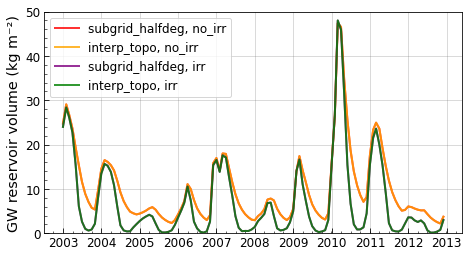
\includegraphics[width=\textwidth]{images/chap3/time_series/cont_slowr_time_series.png}
    \end{subfigure}
        \begin{subfigure}[b]{0.48\textwidth}
        \caption{Groundwater reservoir average seasonal cycle}
        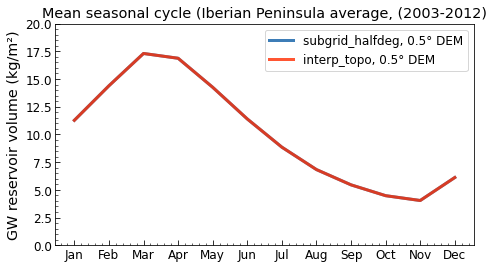
\includegraphics[width=\textwidth]{images/chap3/time_series/cont_slowr_seasonal_cycle.png}
    \end{subfigure} \\
    
    \begin{subfigure}[b]{0.48\textwidth}
        \caption{Overland reservoir average}
        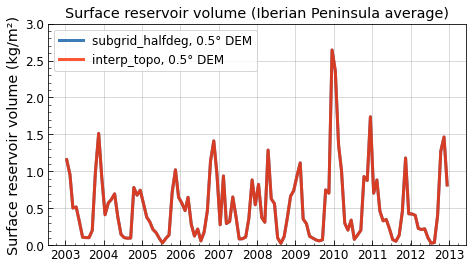
\includegraphics[width=\textwidth]{images/chap3/time_series/cont_fastr_time_series.png}
    \end{subfigure}
    \begin{subfigure}[b]{0.48\textwidth}
        \caption{Overland reservoir average seasonal cycle}
        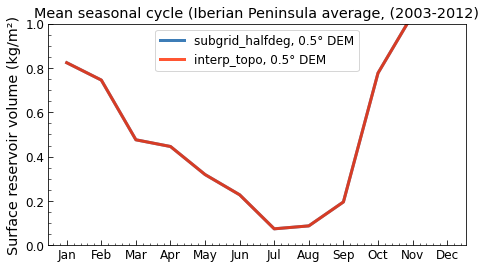
\includegraphics[width=\textwidth]{images/chap3/time_series/cont_fastr_seasonal_cycle.png}
    \end{subfigure} \\
    
    \begin{subfigure}[b]{0.48\textwidth}
        \caption{River reservoir average}
        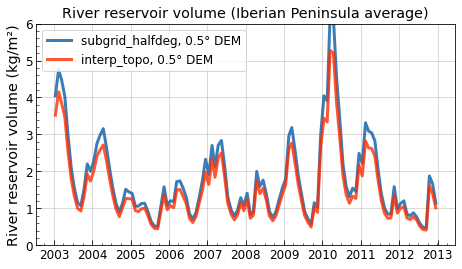
\includegraphics[width=\textwidth]{images/chap3/time_series/cont_streamr_time_series.png}
    \end{subfigure} 
    \begin{subfigure}[b]{0.48\textwidth}
        \caption{River reservoir average seasonal cycle}
        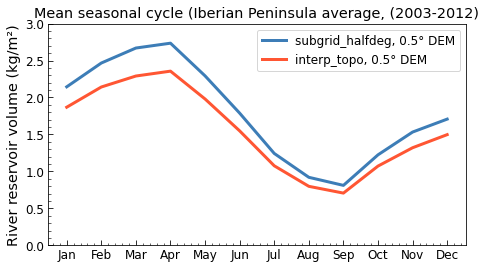
\includegraphics[width=\textwidth]{images/chap3/time_series/cont_streamr_seasonal_cycle.png}
    \end{subfigure} \\

    \caption{Time series and seasonal cycles of reservoir volumes on average over the non-coastal grid cells of the Iberian Peninsula domain.}
    \label{fig:reservoir_cont_time_series}
\end{figure}

\subsection{Simulated irrigation and river discharge}

In the \irr simulations (purple and green lines in Fig. \ref{fig:reservoir_cont_time_series}), all reservoirs are partly depleted by the irrigation withdrawals with both \std and \native, as expected. 
For the groundwater and overland reservoirs, there are still not differences between the two routing if coastal grid cells are excluded, meaning that irrigation has the same with both routing schemes. In general, coastal grid cells are mainly not affected by irrigation since these areas are seldom intensely irrigated.
Regarding the river reservoir (Fig. \ref{fig:reservoir_cont_time_series}f), \std simulates much lower volumes in \irr than in \noirr (-75\% in winter and complete depletion in summer). This decrease is also seen with \native, and the differences between the two routing versions almost disappear in the  \irr simulations, meaning that all the additional river water available in \std is used by the irrigation parameterization. 
When irrigation is activated no matter the routing scheme used, the river reservoir is at its minimum, especially in the large river valleys. Therefore, the discrepancies due to the routing graph have much less impact on the average volume over the domain.

%figure : 3 maps of simulated irrigation (subgrid, interp, diff), TS and SC of irrig for both simulations
\begin{figure}[htbp]
    \centering
    \begin{subfigure}[b]{0.48\textwidth}
        \caption{Irrigation annual mean\\(\std)}
        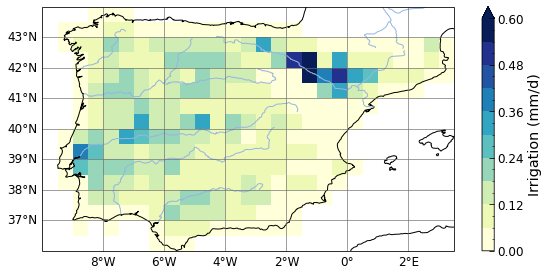
\includegraphics[width=\textwidth]{images/chap3/maps/irrigation_subgrid.png}
    \end{subfigure}
    \begin{subfigure}[b]{0.48\textwidth}
        \caption{Irrigation annual mean\\(\native)}
        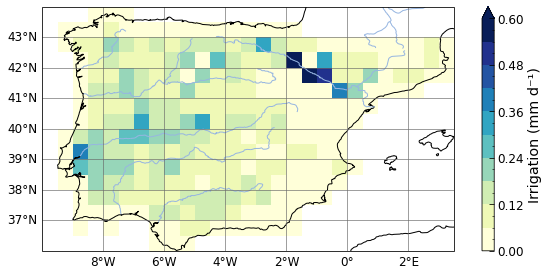
\includegraphics[width=\textwidth]{images/chap3/maps/irrigation_interp.png}
    \end{subfigure} \\
    
    \begin{subfigure}[b]{0.48\textwidth}
        \caption{Irrigation difference\\(\native -\std)}
        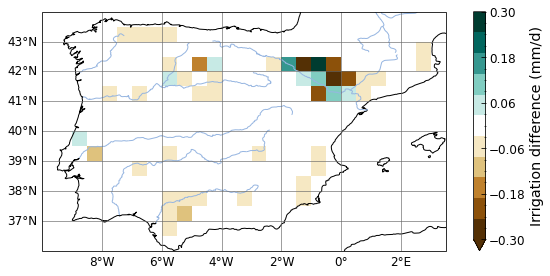
\includegraphics[width=\textwidth]{images/chap3/maps/irrigation_diff.png}
    \end{subfigure} 
    \begin{subfigure}[b]{0.48\textwidth}
        \caption{Irrigation relative difference\\(\native -\std)}
        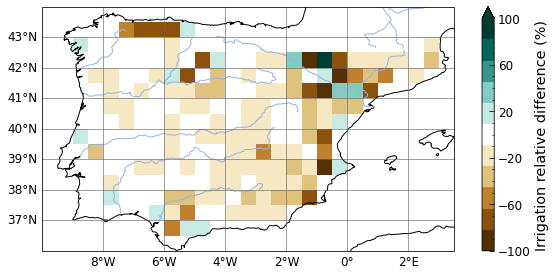
\includegraphics[width=\textwidth]{images/chap3/maps/irrigation_reldiff.png}
    \end{subfigure} \\

    \begin{subfigure}[b]{0.48\textwidth}
        \caption{Irrigation (Iberian Peninsula average)}
        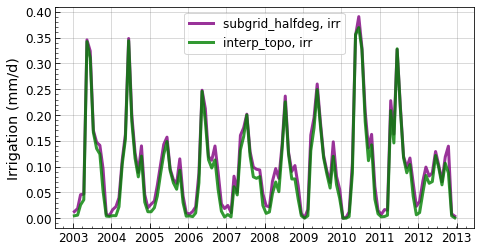
\includegraphics[width=\textwidth]{images/chap3/time_series/irrigation_time_series.png}
    \end{subfigure}    
    \begin{subfigure}[b]{0.48\textwidth}
        \caption{Irrigation average seasonal cycle}
        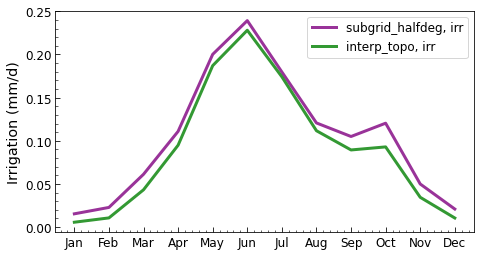
\includegraphics[width=\textwidth]{images/chap3/time_series/irrigation_seasonal_cycle.png}
    \end{subfigure}

    \caption{Simulated irrigation in \std and \native. Annual mean for both simulations (a,b), absolute and relative difference (c-d). Average time series (e) and seasonal cycle (f) over the Iberian Peninsula.}
    \label{fig:irrigation_halfdeg_eval}
\end{figure}

Both simulations show a similar simulated irrigation (Fig. \ref{fig:irrigation_halfdeg_eval}), but the differences on reservoir volumes affect the available water, and therefore irrigation. This is particularly visible in the Ebro valley where some grid cells are highly irrigated in one simulation and not in the other. This is due to the aforementioned differences in the routing network, which affect the path of the Ebro river (Fig. \ref{fig:irrigation_halfdeg_eval}c-d), the main source for irrigation withdrawals in the region (Fig. \ref{fig:irrig_inputs}b).
On average over the domain (Fig. \ref{fig:irrigation_halfdeg_eval}e-f) \std exhibits slightly higher volumes of irrigation than \native (0.103 mm \perday on annual average for \std and 0.090 mm \perday for \native), which is consistent with the higher volumes in the river reservoir. 
As previously mentioned, the differences seen in the reservoirs on coastal grid cells seem to have little impacts on the irrigated volumes, since these regions are seldom intensely irrigated (Fig. \ref{fig:irrig_inputs}a). 

In both simulations, irrigation progressively increases in spring, decreases in July and August, before increasing once again in autumn (Fig. \ref{fig:irrigation_halfdeg_eval}f). Although this section does not aim to provide an in-depth evaluation of the simulated irrigation, it must be noted that this two-peak seasonal cycle is not realistic and does not reflect the irrigation demand, which is highest in July and August. 
This drop in irrigation in summer can be explained by a lack of available water in the routing reservoirs, which are depleted by the end of June (Fig. \ref{fig:reservoir_cont_time_series}). Even though demand remains high, irrigation can not be sustained all summer, and it is only in autumn, when reservoirs are partly replenished by precipitation, that the irrigation demand can once again be satisfied. This aspect was a first hint that the irrigation parametrization might have to be adjusted to better reflect irrigation over the study area, which is further discussed in Section \ref{sec:forcing_irr_reduced}.
An evaluation of simulated irrigation in the Ebro valley is later presented in Section \ref{sec:article1} for the coupled LAM simulations, which were run with the MERIT DEM and a new set of routing parameters determined in Section \ref{section:calib}. 
The Ebro basin the irrigation estimate of \citet{dari_regional_2023} used in Section \ref{sec:article1} has a yearly average value of 0.22 mm \perday over the 2016-2019 period. As a first comparison over the same domain as this product, \std simulates a yealry average of 0.26 mm \perday, and \native of 0.20 mm \perday for the period 2003-2012, confirming that the ORCHIDEE irrigation scheme is in the right order of magnitude.

%figure : river discharge seasonal cycle for 4 stations (large rivers but not Guadalquivir...), 2 routing versions, irr and no_irr for each
\begin{figure}[htbp]
    \centering
    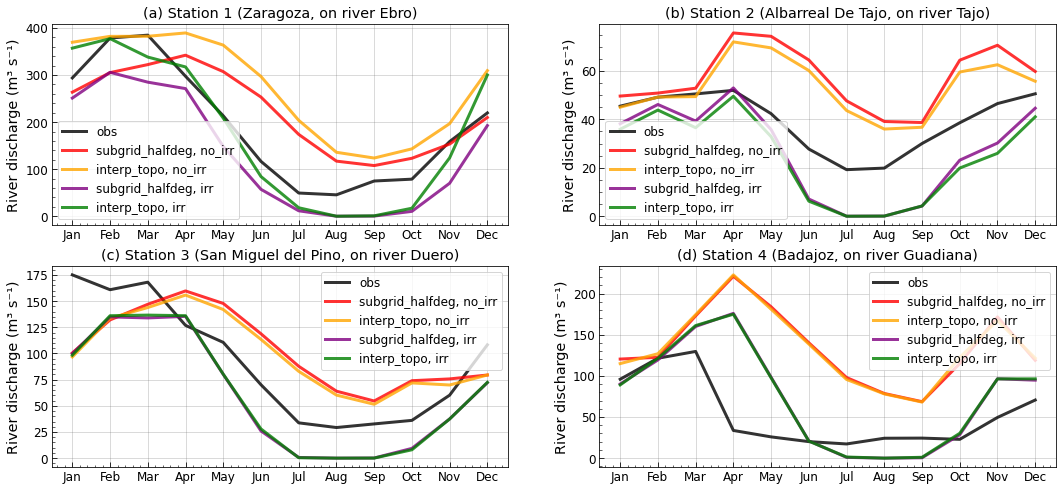
\includegraphics[width=\textwidth]{images/chap3/river_discharge/halfdeg_4stations_SC.png}
    \caption{Mean seasonal cycle (2003-2012) of river discharge in GRDC observations and four simulations, with \native and \std, each with and without irrigation.}
    \label{fig:halfdeg_stations_SC}
\end{figure}

The seasonal cycle of river discharge reflects the general agreement of the two routing versions \ref{fig:halfdeg_stations_SC}. Differences in river discharge are small in most cases, whether irrigation is turned off (red and yellow lines) or activated (purple and green lines). Some differences persist, due to the differences in the routing network already described, mostly for the Ebro river since the station is downstream of several important discrepancies visible on Fig. \ref{fig:routing_reservoirs_halfdeg}l. 

Important limitations of the ORCHIDEE routing scheme (independent of the version used) can already be noticed: without irrigation, river discharge is generally overestimated in these large rivers, and the used irrigation parametrization can not improve this in all seasons since it is mainly inactive when the simulated LAI is low. In reality, water is stored in winter and spring using dams, which explains why the observed discharge is lower than the simulated one, and this water can be used for irrigation in summer, without depleting rivers as much as the irrigation parametrization used here. These aspects will be further discussed in coupled simulations of Chapter \ref{chap:monthly}, using the MERIT DEM and the new set of parameters for the \native routing scheme identified in Section \ref{section:calib}.

\subsection{Conclusions on \native routing consistency}
This comparison of the \native routing version with \std showed that this new version is generally reproducing the modelling principles correctly, though several differences were identified between the two versions:
\begin{itemize}
    \item All three reservoirs are handled differently in \native on coastal grid cells, which affects the average volumes stored over the Iberian Peninsula, but does not have a significant impact on irrigation nor river discharge. 
    \item Differences in the path followed by water as it flows from one grid cell to another through the river reservoirs are also clearly identified in large rivers of the Peninsula. This leads to local changes in the simulated river discharge, and slightly less water stored in the river reservoirs by \native due to shorter paths in several occurrences. These discrepancies have a local impact on irrigation since it is strongly reliant on the volumes of water available in the river reservoir, but this impact remains very limited on average over the domain.
\end{itemize}

\section{Parameter tuning over the Iberian Peninsula}
\label{section:calib}

\subsection{General strategy}

Once the general consistency of the \native routing had been assessed, it became possible to run simulations with the routing scheme setup that would be used for the regional coupled simulation, using the MERIT DEM at 2-kilometre resolution and accounting for irrigation. To use irrigation, the routing time step must be the same as the time step of ORCHIDEE, which is 15 min (900 s) in coupled simulations. 
Differences were quickly noticed when changing the spatial and temporal resolution of the routing scheme compared to those in Section \ref{sec:routing_consistency}, justifying the need for a new set of routing parameters. The objective was to identify parameter values that could enable a study of the impacts of irrigation in coupled ICOLMDZOR simulations, rather than performing an in-depth calibration of the routing scheme. Searching for an optimal parameter set would have required much more specific data collection work to define appropriate metrics, and would likely have been limited by the existing biases of the water budget in ORCHIDEE. 

The parameter tuning pursued three objectives:
\begin{itemize}
    \item Ensuring that simulated volumes in all three river reservoirs were large enough to sustain the irrigation demand.
    \item Reproducing a correct seasonal cycle of river discharge with the \native routing and MERIT DEM.
    \item Adjusting the irrigation withdrawals to better match regional practices of irrigation and ensure a realistic behaviour of river discharge and irrigation, particularly in summer.
\end{itemize}

It was focused on the three time constants of the routing reservoirs (TCST\_SLOW, TCST\_FAST, TCST\_STREAM) and on the \betairrig parameter of the irrigation scheme. This parameter defines the target soil moisture and was already identified in \citet{arboleda-obando_validation_2024} as the most sensitive parameter of the irrigation scheme, pointing out that it might have to be adapted to the region studied.  

ORCHIDEE offline simulations using the \native routing and MERIT DEM were first compared to similar simulations wiht the \std routing and 0.5° DEM to assess reservoir volumes. As a reminder, the irrigation scheme presented in \citet{arboleda-obando_validation_2024} was evaluated and tuned with the \std routing and 0.5° DEM, which explains why it consitutes a relevant reference. 
Simulations were also compared to observations to assess the seasonal cycle of river discharge and the influence of irrigation on summer discharge.

\subsection{Choice of time constants}

At the beginning of this work, three different sets of TCST parameters (presented in Table \ref{table:tcst_refs}) had been used in three different reference studies, each with one of three routing schemes:
\begin{itemize}
\item The values established during an initial calibration of the \native routing performed over the Danube basin with the MERIT DEM, which focused only on river discharge observations \citep{kilic_evaluation_2023}.
\item The default values used by the \std routing on a global scale, which were used in the previous section with the 0.5° DEM. These values were identified empirically by a calibration study over the Senegal river basin and validated globally at 1° resolution in \citet{ngo-duc_53-year_2005, ngo-duc_validation_2007} using river discharge and groundwater measurements from Gravity Recovery and Climate Experiment (GRACE) satellite data.
\item The values used over France with the \textit{subgrid\_HTU} routing and the 2-km input DEM \citep{rinchiuso_improving_2022, huang_multi-objective_2024}.
\end{itemize}

\begin{table}[h]
\centering
\begin{tabular}{|l|c|c|c|}
\hline
\textbf{} & \textbf{TCST\_SLOW} & \textbf{TCST\_FAST} & \textbf{TCST\_STREAM} \\ \hline
Initial \native calibration & 12 & 9 & 0.03 \\ \hline
\std default values & 25 & 3 & 0.24 \\ \hline
\textit{subgrid\_HTU} calibration & 600 & 80 & 6.3 \\ \hline
\end{tabular}
\caption{Reference parameter sets considered to calibrate the \native routing ($day \cdot km^{-1}$).}
\label{table:tcst_refs}
\end{table}

In all three TCST sets, the time constants are separated by approximately an order of magnitude, but the sets themselves exhibit very significant differences from one another (one or two orders of magnitude). 
This can be explained by the different DEMs used, the way HTUs are defined, the calibration choices that led to these sets of values, and also maybe by differences in the code wrapping the physical core of the routing, which is not the same in the three routing schemes, and inclued pretreatments of the DEM to aggregate topographic indices in \std and \textit{subgrid\_HTU}.
To simplify this parameter space, three TCST sets were defined, to approach the values of the reference sets of Table \ref{table:tcst_refs} while respecting the following ratios:
\begin{equation}
    TCST\_SLOW = 10 \times TCST\_FAST = 100 \times TCST\_STREAM.
\end{equation}

This means that the residence time in the groundwater reservoir is 10 times larger than the residence time of the overland reservoir, and 100 times larger than the residence time in the stream reservoir, which makes sense hydrologically.
Table \ref{table:tcst_exp} presents these three parameter sets (TCST1, TCST2, TCST3), as well as the parameter set eventually selected after the parameter tuning (TCST4). This choice is justified hereafter, based on the results of the four simulations that were carried out with these four TCST sets (simulations without irrigation using the WFDEI meteorological forcing over 2003-2012 after warm-up). 

\begin{table}[h]
\centering
\begin{tabular}{|l|c|c|c|}
\hline
\textbf{} & \textbf{TCST\_SLOW} & \textbf{TCST\_FAST} & \textbf{TCST\_STREAM} \\ \hline
TCST1 & 3 & 0.3 & 0.03 \\ \hline
TCST2 & 30 & 3 & 0.3 \\ \hline
TCST3 & 300 & 30 & 3 \\ \hline
TCST4 & 700 & 100 & 0.1 \\ \hline
\end{tabular}
\caption{Value sets of the simulations for the parameter tuning of the \native routing ($day \cdot km^{-1}$).}
\label{table:tcst_exp}
\end{table}

The volumes in each of the reservoirs were first compared to the volumes simulated by the \std routing. As a reminder, this version, with the 0.5° DEM, has long been used in ORCHIDEE and was evaluated against groundwater reference products from GRACE, as well as river discharge observations  \citep{ngo-duc_53-year_2005, ngo-duc_validation_2007}.
It is also the version that was used for the evaluation and validation of the irrigation scheme at global scale \citep{arboleda-obando_validation_2024}, which makes it a relevant reference for the reservoir volumes since available water is a major driver of simulated irrigation in the model. 

On average over the Peninsula, for the groundwater and overland reservoirs, the TCST3 simulation showed values closest to \std (Fig. \ref{fig:reservoir_time_series_tcsts}a-d), while TCST1 and TCST2 hold almost no water in these reservoirs, as they flow more quickly in the river reservoir. 
For the river reservoir however (Fig. \ref{fig:reservoir_time_series_tcsts}e-f), TCST3 is one order of magnitude above the other simulations, including \std, hinting that water circulates too slowly, \textit{i.e.}  TCST\_STREAM is too large for this reservoir in TCST3. This is confirmed looking at river discharge (Fig. \ref{fig:merit_tcsts_stations_SC}), as TCST3 cannot reproduce the observed structure of the seasonal cycle for any of the four rivers considered, due to a large phase lag. 

These results, as well as a few intermediate tests not shown here, led to the choice of a new set of parameters (TCST4 in Table \ref{table:tcst_exp}), which has values similar to TCST3 for the groundwater and overland reservoirs, but reduced TCST\_STREAM (closer to TCST2, and even slightly faster), shown in red in Fig. \ref{fig:reservoir_time_series_tcsts} and \ref{fig:merit_tcsts_stations_SC}.
Average simulated volumes for TCST4 are close to \std for all reservoirs, and match discharge observations with similar performance to TCST1 and TCST2.
%todo:add metrics ? KGE, BIAS
It can be noted that the performance of TCST1 for river discharge is good, but that it holds almost no water in the groundwater and overland reservoirs, suggesting that this previous calibration with the 2-km MERIT DEM which focused only on matching discharge observations \citep{kilic_evaluation_2023} neglected some aspects of the routing scheme and effectively calibrated only TCST\_STREAM.

Using the new set of parameters TCST4 for the routing scheme, the sensitivity of simulated river discharge to irrigation was then explored, as well as the influence of the atmospheric forcing used for the offline simulations.

%figure : 3 time series (3 reservoirs) on average over the IP for 4 tcsts and std as reference
\begin{figure}[htbp]
    \centering
    \begin{subfigure}[b]{0.48\textwidth}
        \caption{Groundwater reservoir average}
        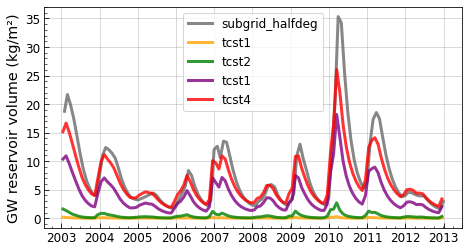
\includegraphics[width=\textwidth]{images/chap3/time_series/slowr_time_series_tcsts.png}
    \end{subfigure}
    \begin{subfigure}[b]{0.48\textwidth}
        \caption{Groundwater reservoir average seasonal cycle}
        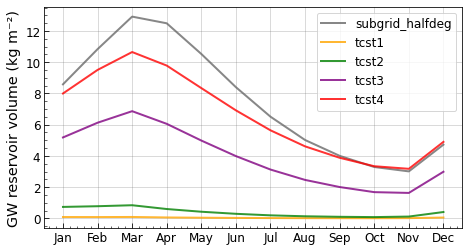
\includegraphics[width=\textwidth]{images/chap3/time_series/slowr_seasonal_cycle_tcsts.png}
    \end{subfigure} \\
    
    \begin{subfigure}[b]{0.48\textwidth}
        \caption{Overland reservoir average}
        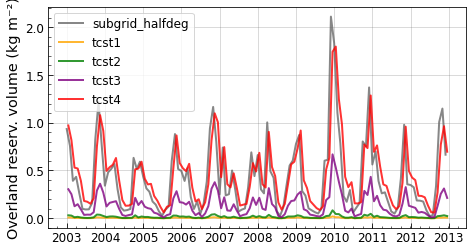
\includegraphics[width=\textwidth]{images/chap3/time_series/fastr_time_series_tcsts.png}
    \end{subfigure}
    \begin{subfigure}[b]{0.48\textwidth}
        \caption{Overland reservoir average seasonal cycle}
        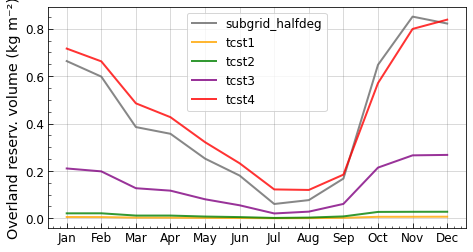
\includegraphics[width=\textwidth]{images/chap3/time_series/fastr_seasonal_cycle_tcsts.png}
    \end{subfigure} \\
    
    \begin{subfigure}[b]{0.48\textwidth}
        \caption{River reservoir average}
        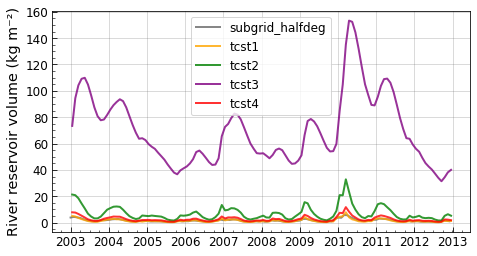
\includegraphics[width=\textwidth]{images/chap3/time_series/streamr_time_series_tcsts.png}
    \end{subfigure} 
    \begin{subfigure}[b]{0.48\textwidth}
        \caption{River reservoir average seasonal cycle}
        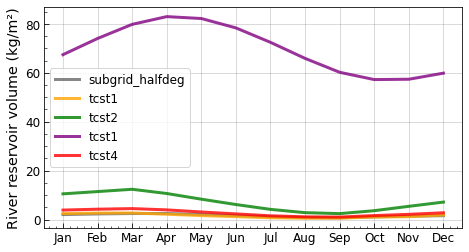
\includegraphics[width=\textwidth]{images/chap3/time_series/streamr_seasonal_cycle_tcsts.png}
    \end{subfigure} \\

    \caption{Time series and seasonal cycles of reservoir volumes on average over the Iberian Peninsula domain (WFDEI forcing, 2003-2012).}
    \label{fig:reservoir_time_series_tcsts}
\end{figure}

%figure : river discharge seasonal cycle for 4 stations (large rivers but not Guadalquivir...), 2 routing versions, irr and no_irr for each
\begin{figure}[htbp]
    \centering
    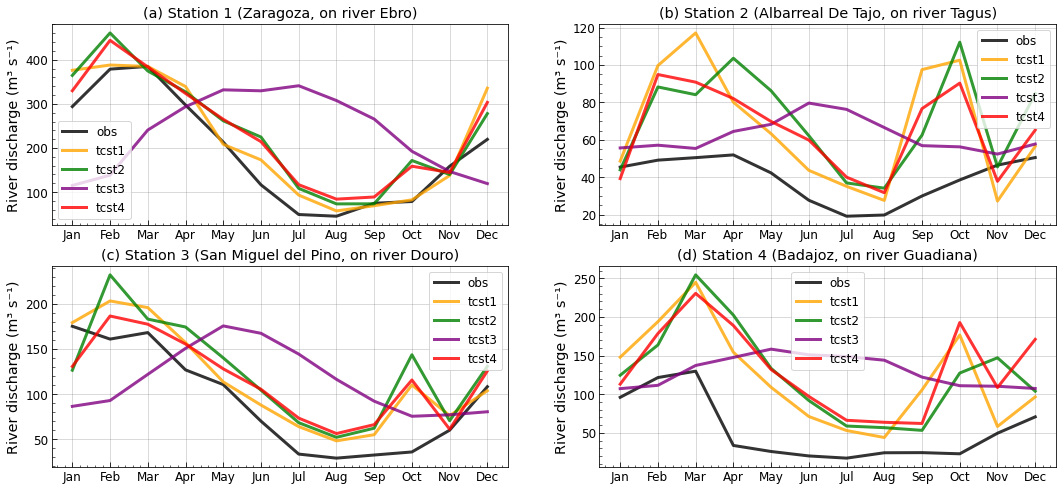
\includegraphics[width=\textwidth]{images/chap3/river_discharge/merit_tcst_4stations_SC.png}
    \caption{River discharge mean seasonal cycle (WFDEI forcing, 2003-2012) with four sets of TCST parameters.}
    \label{fig:merit_tcsts_stations_SC}
\end{figure}

\clearpage

\subsection{Irrigation parameter tuning}
\label{sec:forcing_irr_reduced}

\begin{figure}[htbp]
    \centering
    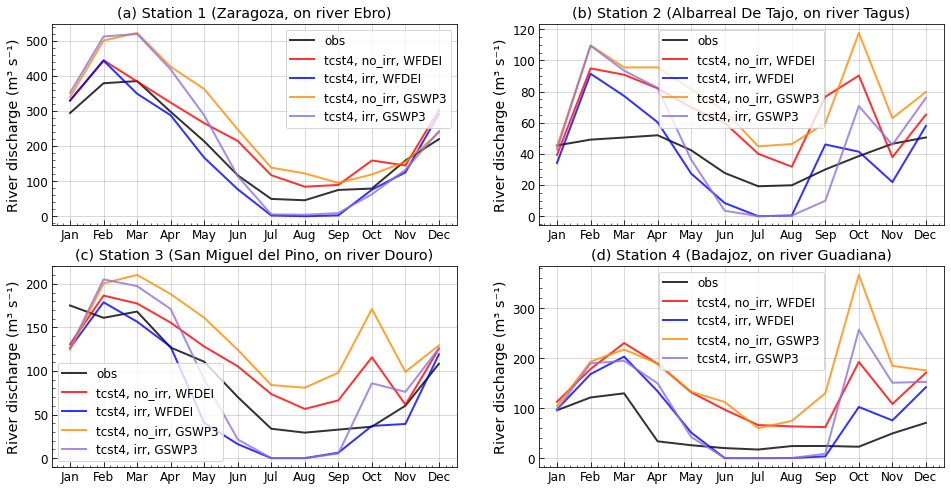
\includegraphics[width=\textwidth]{images/chap3/river_discharge/merit_forcing_4stations_SC.png}
    \caption{River discharge mean seasonal cycle (2003-2010) with GSWP3 and WFDEI forcings, with and without irrigation.}
    \label{fig:merit_forcing_stations_SC}
\end{figure}

The first goal was to assess if the activation of irrigation had the potential to improve the simulated river discharge. This was jointly analysed with the impacts of the atmospheric forcing, which is known to bring significant uncertainties in the simulated variables in forced mode \citep{gelati_hydrological_2018,boone_land_2025}.
To this end,  four simulations were performed, all with the TCST4 parameter set, using two atmospheric forcings (WFDEI and GSWP3), each with and without irrigation. Considering the availability of GSWP3, the simulations were only run until 2010, and analysed over 8 years (2003-2010).

The results (Fig. \ref{fig:merit_forcing_stations_SC}) show a response to both changes but a stronger impact of irrigation, which strongly reduces discharge, except in winter. The WFDEI and GSWP3 forcing produce seasonal cycles with similar structures but using the GSWP3 forcing leads to larger peak discharge, in winter for the Ebro and Douro basin, as well as in autumn, a period of high precipitation in the Tagus, Douro and Guadiana basins. These regional and seasonal specificities reflect the differences in precipitation between the two forcings. 
%option:show yearly or seasonal maps of precip ? side by side, diff ?
In summer, the \noirr and \irr simulations with the two forcings are similar, especially with irrigation, which depletes the river reservoir, reducing discharge to near-zero for the four rivers.

The strengths of these responses, much larger than the differences induced by the TCST sets explored in Fig. \ref{fig:merit_tcsts_stations_SC}, justified the decision not to pursue finer tuning of the TCST parameters, which would be too dependent on the forcing or the activation of irrigation. The TCST4 parameter set was considered an acceptable option for the routing scheme, and it was decided to expand the parameter tuning to include the parametrization of irrigation. 

\begin{figure}[htbp]
    \centering
    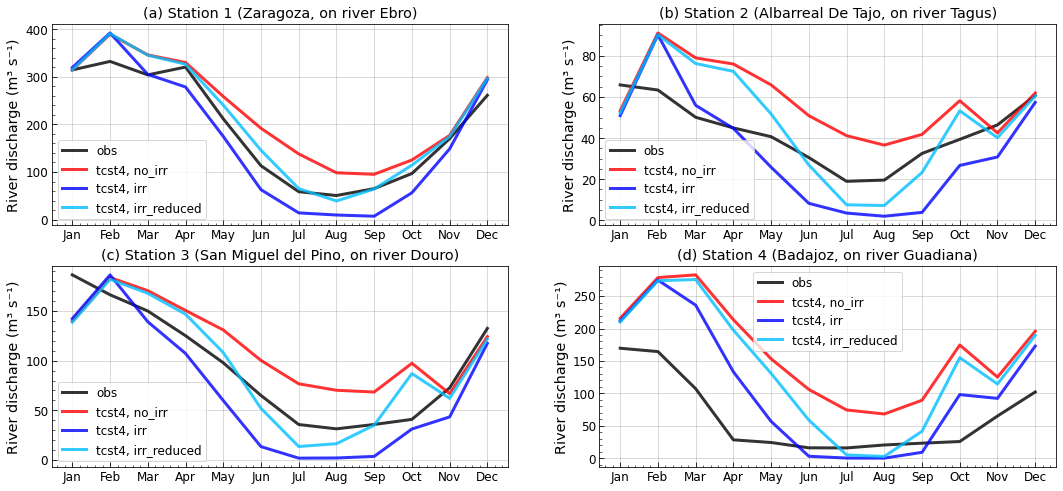
\includegraphics[width=\textwidth]{images/chap3/river_discharge/merit_irr_4stations_SC.png}
    \caption{River discharge mean seasonal cycle  in the \noirr, \irr and \textit{irr\_reduced} simulations (WFDEI forcing, 2003-2012).}
    \label{fig:merit_irr_stations_SC}
\end{figure}

\hfill

The global evaluation of the ORCHIDEE irrigation scheme \citep{arboleda-obando_validation_2024} identified the \betairrig parameter as the main driver of the simulated irrigation. This parameter conditions the soil moisture target as a fraction of soil moisture at field capacity. The default value selected for global simulations was \betairrig = 0.9, meaning the irrigation scheme aims at keeping soil moisture in the root zone at 90 \% of the field capacity moisture. But this value was selected as a way to centre the global biases compared to reference products on zero, acknowledging that this value was too low for some regions and too high for others. In other words, this \betairrig value was chosen as an effective value for the global scale, meant to reflect a large diversity of irrigation practices, including flooding methods in rice paddies, which is common in intensely irrigated regions of northern India and China. As explored in \citet{arboleda-obando_validation_2024}, \betairrig = 1.2 would be more appropriate to represent the irrigation withdrawals properly for such practices. In the Iberian Peninsula, in contrast, the limited water supply and semi-arid climate favour less water intensive methods (drip or sprinkler irrigation) which would be better represented with lower values of \betairrig. 

This is why other values were explored over the Iberian Peninsula, in particular to limit the unrealistic depletion of rivers in summer. Fig. \ref{fig:merit_irr_stations_SC} shows three simulations, all with the WFDEI forcing and TCST4 set of parameters for routing, but with different options for irrigation: \noirr, \irr (default value \betairrig = 0.9) and \textit{irr\_reduced} with \betairrig = 0.6. 
This simulation limits the depletion in summer and yields much better performance in the Ebro basin, a very intensely irrigated region which largely depends on water from river (as opposed to groundwater) for irrigation (Figure \ref{fig:irrig_inputs}).
This reduced irrigation also seems more consistent when looking at the seasonal cycle of irrigation (Fig. \ref{fig:merit_irr_reduced}c). In the \irr simulation, high volumes are withdrawn in the spring but irrigation drops in summer, which is the season where irrigation demand is the highest. This is due to a lack of available water in the reservoirs in the irrigated regions in summer, which are depleted too quickly when using \betairrig = 0.9. The effect of the river reservoir depletion is also visible on the summer river discharge of Fig. \ref{fig:merit_irr_stations_SC} which falls to near-zero for the four rivers considered. 

To summarize, the \textit{irr\_reduced} setup simulates a lower demand in irrigation and therefore less irrigation overall, but it avoids an early depletion of the reservoirs, yielding a more consistent seasonal cycle of irrigation and matching discharge observation better in spring and summer. A more quantitative evaluation of the simulated irrigation with \betairrig = 0.6 (in coupled simulations) is proposed in section \ref{sec:irrig_eval} against observations in the Ebro basin.
%option : also show root_deficit to demonstrate that large Beta leads to much larger demand

%figure : maps of irrig in irr and irr_reduced, and seasonal cycle of irrig over IP for both sims
\begin{figure}[htbp]
    \centering
    \begin{subfigure}[b]{0.48\textwidth}
        \caption{Mean irrigation in \irr.\\ } 
        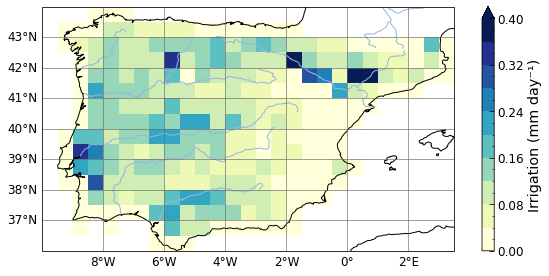
\includegraphics[width=\textwidth]{images/chap3/maps/irrigation_ave_tcst4_irr.png}
    \end{subfigure}
    \begin{subfigure}[b]{0.48\textwidth}
        \caption{Mean irrigation in \textit{irr\_reduced}.} 
        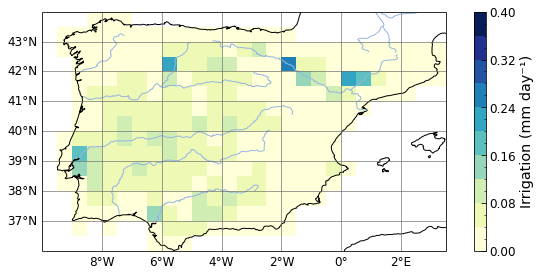
\includegraphics[width=\textwidth]{images/chap3/maps/irrigation_ave_tcst4_irr_reduced.png}
    \end{subfigure} \\

    \begin{subfigure}[b]{0.5\textwidth}        
        \caption{Seasonal cycle of irrigation.} 
        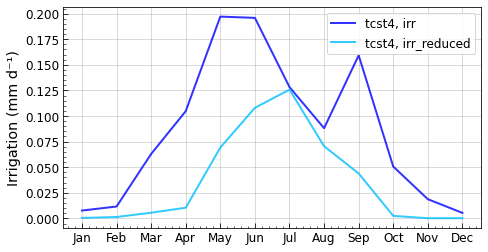
\includegraphics[width=\textwidth]{images/chap3/time_series/irrigation_seasonal_cycle_irr_reduced.png}
    \end{subfigure}
    \caption{Simulated irrigation in the \irr and \textit{irr\_reduced} simulations (WFDEI forcing, 2003-2012).}
    \label{fig:merit_irr_reduced}
\end{figure}

\pagebreak

\section{Chapter conclusions}

This chapter presents the evaluation and parameter tuning of the new version of the routing scheme (\native) using ORCHIDEE offline simulations over the Iberian Peninsula. This was a necessary step to prepare for coupled simulations; It provided a finer understanding of the behaviour of the routing scheme with different DEMs, and also highlighted the interdependency between the irrigation parametrization, the routing reservoirs, and river discharge. 

This work first showed that the new routing code mostly behaves similarly to the pre-existing version (\std) if given the same time step, input map (0.5° DEM), and parameters, although some differences were identified, mostly on the coastal grid cells. In non-coastal grid cells, differences in the routing path also appeared between \std and \native, leading to local differences in discharge and irrigation.

The \native routing was then used with a high-resolution (2 km) DEM over the Iberian Peninsula, and several options were tested for the reservoir time constants, leading to the choice of parameter set TCST4.The simulation with this parameter set presents a correct river discharge seasonnal cycle for the major rivers of the Peninsula, while maintaining sufficient water volumes in the groundwater and overland reservoirs. 
This aspect was essential because of the dependence of the irrigation scheme on the available water in the routing reservoirs.
This parameter tuning underlined the limits of a previous calibration by \citet{kilic_evaluation_2023} and of the default values inherited from the \std routing regarding the groundwater and overland reservoirs.

Sensitivity experiments also highlighted the very large response of river discharge to the activation of irrigation (except in winter), and a significant yet more moderate response to the atmospheric forcing used for the parameter tuning. 
The magnitude of these sensitivities also contributed to the decision not to further calibrate the TCST values, as their impact on simulated river discharge performance remains limited compared to that of irrigation.
As a consequence, alternative options were explored for the \betairrig parameter of the irrigation scheme, and 0.6 was identified as a more suitable value than the default value of 0.9. This option limits depletion of the reservoirs, which makes the seasonal cycle of irrigation more consistent and enables better agreement with discharge observations in summer. As hypothesized in \citet{arboleda-obando_validation_2024} this value is considered more consistent with a representation of irrigation practices in semi-arid regions.

Therefore, coupled simulations presented in Chapter \ref{chap:monthly} were both run using the TCST4 set of routing parameters, and \betairrig = 0.6 for the \irr simulation.
